% A single-column paper in the layout of NeurIPS's style — made up — with
% what Reflow once read badly in one: a byline set with wide spaces, its
% notes as footnotes and its addresses as one group; links boxed; a figure
% clipped out of a larger drawing under a paragraph; two-level scripts in a
% line of text; tables captioned under them, one over another, with group
% labels set sideways and a heading spanning its columns by a rule; tables
% side by side; heading cells on several lines; a label across four
% columns; and a bold "A.5" heading straight over a table.
% Rebuilt with: pdflatex neurips-single-column-figure.tex && pdflatex neurips-single-column.tex
% (texlive-latex-recommended).
\documentclass[10pt]{article}
\usepackage[margin=1.5in]{geometry}
\usepackage{amsmath,amssymb,booktabs,graphicx,xcolor,float}
\usepackage{hyperref}
\title{\textbf{Small Models by Pruning and Distillation}}
\author{\textbf{Ada Lindqvist}\thanks{Equal contribution.} \hspace{2.2em} \textbf{Tomas Okafor}\footnotemark[1] \hspace{2.2em} \textbf{Mira Castell}\\
\textbf{Ravi Anand} \hspace{2.2em} \textbf{Lena Ferris} \hspace{2.2em} \textbf{Omar Haddad}\\
Northfield Labs\\
\texttt{\{adal,tomaso,mcastell,ranand,lferris,ohaddad\}@northfield.example.org}}
\date{}
\begin{document}
\maketitle
\begin{abstract}
Models are usually trained from scratch at every size. We prune a large model and retrain the smaller ones with a fraction of the data, and they match or beat models trained from scratch at the same size, at a fortieth of the cost.
\end{abstract}
\section{Introduction}
Large models dominate language processing \cite{a,b}. Training a family of them from scratch is costly, so we prune the largest and retrain the rest with distillation \cite{b}. This paragraph goes on long enough to fill several lines of running text, so that the body of the page is measured properly by the reader, and it cites more work \cite{a} as it goes.
\subsection{Importance}
Estimating the importance of neurons, heads and layers is well studied \cite{a,b}. Recent work on pruning language models has focused on gradients \cite{a}, cosine similarity \cite{b} and perplexity \cite{a} on a calibration set, which we compare here.
\begin{figure}[h]
\centering
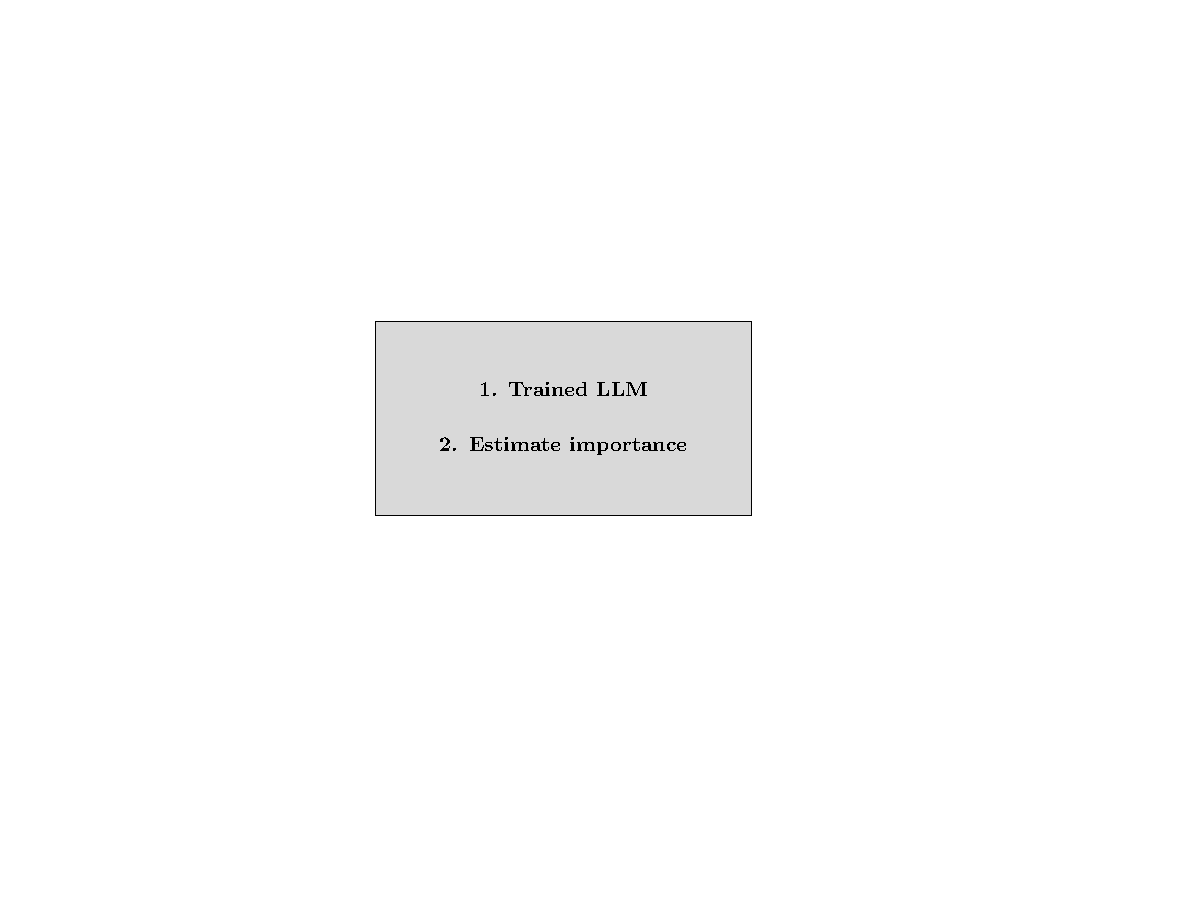
\includegraphics[viewport=170 150 400 290,clip,width=0.7\linewidth]{neurips-single-column-figure.pdf}
\caption{Overview of the approach: the trained model, and the importance estimated.}
\end{figure}
We define the layer as $\mathrm{MLP}(X) = \delta(X W_1^T) W_2$, where $W_1, W_2 \in \mathbb{R}^{d_{hidden}\times d_{model}}$, and $d_{model}$ and $d_{hidden}$ are the embedding and hidden dimensions of the model we prune in the rest of this paper.
\section{Results}
We compare the pruned models with models of their size in the two tables below, and give the chat results after them.
\begin{table}[h]
\centering\footnotesize
\begin{tabular}{llllll}
\toprule
 & & & \multicolumn{3}{c}{Models}\\
\cmidrule(l){2-6}
 & Benchmark & Metric & Base & Mistral & Ours\\
\midrule
 & \# Parameters & & 8B & 7.3B & 8.3B\\
 & \# Tokens & & 15T & 8T & 94B\\
\midrule
\raisebox{-1.6ex}[0pt][0pt]{\rotatebox{90}{Logic}} & winogrande (5) & acc & 77.6 & 78.5 & \textbf{79.0}\\
 & MMLU (5) & acc & 65.3 & 64.1 & 63.8\\
\midrule
\raisebox{-1.6ex}[0pt][0pt]{\rotatebox{90}{Code}} & MBPP (0) & pass@1 & 42.4 & 38.8 & 35.2\\
 & HumanEval (0) & pass@1 & 28.1 & 28.7 & 31.6\\
\bottomrule
\end{tabular}
\caption{Performance of the pruned 8B model against models of its size.}
\end{table}
\begin{table}[h]
\centering\footnotesize
\begin{tabular}{llll}
\toprule
Benchmark & Phi & Gemma & Ours\\
\midrule
MMLU (5) & 57.5 & 42.0 & 58.6\\
HellaSwag (10) & 75.2 & 72.0 & 75.0\\
\bottomrule
\end{tabular}
\caption{Performance of the pruned 4B model against models of its size.}
\end{table}
\begin{table}[h]
\begin{minipage}[b]{0.46\linewidth}\centering\scriptsize
\begin{tabular}{lll}
\toprule
Model & \shortstack[l]{Non-\\Emb.\\Params} & Total\\
\midrule
Ours-instruct & 2.6B & 6.46\\
Phi-chat & 2.5B & 4.29\\
\bottomrule
\end{tabular}
\caption{Results on MT-Bench.}
\end{minipage}\hfill
\begin{minipage}[b]{0.46\linewidth}\centering\scriptsize
\begin{tabular}{ll}
\toprule
Model & Avg.\\
\midrule
Ours-instruct & 53.09\\
Gemma-it & 41.63\\
Llama-instruct & 50.51\\
\bottomrule
\end{tabular}
\caption{Results on BFCL.}
\end{minipage}
\end{table}
\begin{table}[h]
\centering\footnotesize
\begin{tabular}{llllll}
\toprule
DEP & MLP & ATT & EMB & Distillation Loss & LM Val Loss\\
\midrule
$\checkmark$ & $\checkmark$ & $\checkmark$ & $\checkmark$ & 5.35 $\rightarrow$ 0.38 & 2.062\\
$\times$ & $\checkmark$ & $\checkmark$ & $\times$ & 5.07 $\rightarrow$ 0.42 & 2.101\\
\multicolumn{4}{c}{Train from scratch (random init)} & 12.27 $\rightarrow$ 2.34 & 3.953\\
\bottomrule
\end{tabular}
\caption{Pruning strategies before and after retraining.}
\end{table}
\appendix
\section{Appendix}
\subsection{One-shot vs.\ Iterative Pruning}
\begin{table}[H]
\centering\footnotesize
\begin{tabular}{ll}
\toprule
Loss components & LM loss\\
\midrule
logits & 2.155\\
logits + embedding & 2.141\\
\bottomrule
\end{tabular}
\caption{Ablation of the loss components.}
\end{table}
\begin{thebibliography}{2}
\bibitem{a} A. Author, ``A first paper,'' 2023.
\bibitem{b} B. Writer, ``A second paper,'' 2024.
\end{thebibliography}
\end{document}
